\documentclass[12pt]{article} % use 12pt option to have the same font size as Amadeus templates; you can also use smaller fonts (10pt, 11pt) to save space, if you do not mind having a size different from that in Amadeus templates

%\usepackage{verbatim}
%\usepackage{hyperref}
\usepackage{amadeus}
% Possible options:
% arial: to have arial font (it is the case in Amadeus' template)
% confidential or internal: for corresponding logo to be added (it can also be omitted)
%
%%%%%%%%%%%%%%%%%%%%%%%%%%%%%%%%%%%%%%%%%%%%%%%%%%%%%%%%%%%%%%%%%%%%%%%%%%%%%%%%%%%%%%%%%%%
% Path to folders containing graph files (e.g., \graphicspath{{graphs/}, {graphs2/}})
%\graphicspath{{graphs/}}
%%%%%%%%%%%%%%%%%%%%%%%%%%%%%%%%%%%%%%%%%%%%%%%%%%%%%%%%%%%%%%%%%%%%%%%%%%%%%%%%%%%%%%%%%%%
% Packages
%
\usepackage{amsmath}
%%%%%%%%%%%%%%%%%%%%%%%%%%%%%%%%%%%%%%%%%%%%%%%%%%%%%%%%%%%%%%%%%%%%%%%%%%%%%%%%%%%%%%%%%%%
% Shortcuts

%%%%%%%%%%%%%%%%%%%%%%%%%%%%%%%%%%%%%%%%%%%%%%%%%%%%%%%%%%%%%%%%%%%%%%%%%%%%%%%%%%%%%%%%%%%
% Header and footer
% First entry: left header, usually related to the title of the document
% Second entry: department (can be left blank)
% Third entry: usually "Last update: yyyy/mm/dd" (can be left blank)
% Example: \makeheaderandfooter{Title of Document}{Charles-Antoine Robelin}{Last update: 31-May-2011}
\makeheaderandfooter{Airline Market Simulator -- Sequential Discrete Event Generation}{Charles-Antoine Robelin}{Last update: 31-May-2011}
%%%%%%%%%%%%%%%%%%%%%%%%%%%%%%%%%%%%%%%%%%%%%%%%%%%%%%%%%%%%%%%%%%%%%%%%%%%%%%%%%%%%%%%%%%%
\begin{document}
%=====================================================================
%=====================================================================
%=====================================================================
%
% Title and Table of Contents Pages
%
%=====================================================================
%=====================================================================
%=====================================================================
%
% \maketitlepage, with three entries: title, subtitle, and second subtitle (the font size is not available with all fonts, but it should not be too much of a problem)
\maketitlepage{Airline Market Simulator}{Sequential Event Generation}{}
%
\maketableofcontentspage
%
%=====================================================================
%=====================================================================
%=====================================================================
%
% Main Body of Document
%
%=====================================================================
%=====================================================================
%=====================================================================
\mainbody
\vspace*{6cm}
%=====================================================================
%=====================================================================
%
\section{Objective}
%
%=====================================================================
%=====================================================================
The purpose of this note is to describe the generation of arrival
times of events (for example, requests for travel for a given set of
travel attributes, also referred to as instances of travel
demand). More specifically, the generation of arrival times one at a
time, in increasing order, is described here, with the following
assumptions:
\begin{itemize}
\item The number of events is determined a priori (e.g., following any
  distribution)
\item The arrival times of the events should follow an arrival pattern
  that is also given (e.g., determined from historical data).
\end{itemize}
The main result is described in section~\ref{sec:methodtwo}.\par
There are two possibilities for the generation of arrival times:
\begin{itemize}
\item The arrival times of all events are generated at the beginning
  of the simulation and stored in the event queue (the times are
  sorted when being inserted in the event queue); or,
\item The arrival time of the first event is generated and stored in
  the event queue; at the time of the first event, the time of the
  second event is generated and stored in the event queue; and so on
  with all the remaining events. This method can be referred to as
  {\itshape one-at-a-time} or {\itshape sequential} generation.
\end{itemize}
The second option requires less memory space than the first option,
and has been successfully implemented in the case of exponentially
distributed inter-arrival times (i.e., number of events with a Poisson
distribution).\par
The method described in this note also implements the second option,
while accommodating total numbers of events that follow any
distribution (i.e., the variance of the total number of events can be
set to any value).
%
%=====================================================================
%=====================================================================
%
\section{Notations and Assumptions}
%
%=====================================================================
%=====================================================================
The number of events to be generated is denoted by $N$. The arrival
pattern is an increasing function of time $t$ (time to departure in
our example) and is denoted by $A(t)$. The function $A$ is assumed to
take values of 0 at some given time $\tau_\text{init}$ and 1 at time
0, i.e., no events have arrived at time $\tau_\text{init}$ (beginning
of the booking period in the case of demand for travel) and all events
have arrived by time 0 (date of the flight in the case of demand for
travel). The function $A$ is also assumed to be invertible, with
inverse $A^{-1}$. An example of arrival pattern $A$ is shown in
figure~\ref{fig:arrivalPattern}.
\begin{figure}[h`!]
\centering
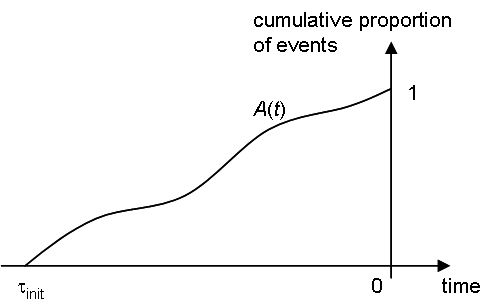
\includegraphics{arrivalPattern}
\vspace{-4mm}
\caption{Example of arrival pattern.}
\label{fig:arrivalPattern}
\end{figure}
%
%=====================================================================
%=====================================================================
%
\section{Reduction of the Problem to the Generation of Uniformly Distributed Variates}
%
%=====================================================================
%=====================================================================
The objective is to generate $N$ arrival times $t_1,\ \ldots,\ t_N$
between $\tau_\text{init}$ and 0, following the arrival pattern
described by $A$. This can be obtained by\footnote{See, for instance,
  Wikipedia's entry on how to generate random samples from a probability
  distribution
  (http://en.wikipedia.org/wiki/Random\_generator\#Generation\_from\_a\_probability\_distribution)}:
\begin{itemize}
\item generating $N$ variates $x_1,\ \ldots,\ x_N$, each of which is
  uniformly distributed between 0 and 1,
\item taking $t_i = A^{-1}(x_i)$ for each $i$ (this can be seen as a
  projection, as shown in figure~\ref{fig:projection} where $N=3$).
\end{itemize}
\begin{figure}[ht]
\centering
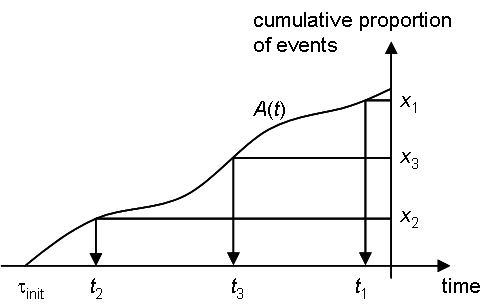
\includegraphics{projection}
\vspace{-4mm}
\caption{Determination of $t_i$'s from $x_i$'s.}
\label{fig:projection}
\end{figure}
Note that there is no reason for the $x_i$'s (or the $t_i$'s) to be
ordered. Therefore, all the $x_i$'s must be generated at the beginning
of the simulation, and the corresponding $t_i$'s are stored in the
event queue. Alternatively, it would be desirable to ``generate the
$x_i$'s in increasing order, one at a time,'' in order to save memory
space. This problem will be formulated in a more formal manner and
addressed in section~\ref{sec:justification}.
%
%=====================================================================
%=====================================================================
%
\section{Generation Methods}\label{sec:generation}
%
%=====================================================================
%=====================================================================
As mentioned earlier, the number $N$ of requests is assumed to be
given, and the arrival pattern is described by a given function $A$
(with inverse $A^{-1}$). The two methods described below generate a
set of $N$ arrival times. The management of the event queue is also
described, in order to show the difference between the two methods.
%
%=====================================================================
%
\subsection{Method 1: All-at-Once Generation}\label{sec:methodone}
%
%=====================================================================
\begin{verbatim}
for i from 1 to N:
    x[i] <- rand    # rand: returns a random number between 0 and 1
end for
for i from 1 to N:
    t[i] <- inverse_of_A(x[i])
    place t[i] in event queue  # the event queue automatically sorts the events
end for
retrieve events from the event queue when necessary and
            handle these events
\end{verbatim}
In this method, all times $t_i$'s are generated at the beginning of
the simulation and stored in the event queue, which automatically
sorts them (by arrival times).
%
%=====================================================================
%
\subsection{Method 2: One-at-a-Time Generation or Sequential Generation}\label{sec:methodtwo}
%
%=====================================================================
\begin{verbatim}
pr_x <- 0
for k from 1 to N:
    x <- 1-(1-pr_x)*(1-rand)^(1/(N-k+1))  # rand: returns a random number
                                          #       between 0 and 1
    pr_x <- x
    t <- inverse_of_A(x)
    place t in event queue
    retrieve t when necessary and handle event
end for
\end{verbatim}
The formula \verb#1-(1-pr_x)*(1-rand)^(1/(N-k+1))# will be derived
in section~\ref{sec:justification}. In this method, the times $t_i$'s
are generated one at a time in increasing order, which requires less
memory space than for the first method. The distribution of the
$x_i$'s, and thus of the $t_i$'s, is the same for both methods (after
sorting them for method 1, which is done when they are placed in the
event queue). This result is justified in
section~\ref{sec:justification}.
%
%=====================================================================
%=====================================================================
%
\section{Justification of the Equivalence of Both Generation Methods in Terms of Distribution of Arrival Times}\label{sec:justification}
%
%=====================================================================
%=====================================================================
%
%=====================================================================
%
\subsection{Order Statistic}
%
%=====================================================================
The $k$-th order statistic of a statistical sample is its $k$-th
smallest value, and is usually denoted by $X_{(k)}$. For example, let
us consider the following sample of size 3:
\[
x_1=0.8,\ x_2=0.2,\ x_3=0.6
\]
where the indices only represent the order in which the numbers were
drawn and are not important (this is the case for our
application). The order statistics are as follows:
\[
x_{(1)}=0.2,\ x_{(2)}=0.6,\ x_{(3)}=0.8
\]
$X_{(1)}$ is the first order statistic and is the minimum of the sample, i.e.,
\[
X_{(1)}=\min\{X_1,X_2,\ldots,X_n\}
\]
where $n$ is the sample size. $X_{(n)}$ is the $n$-th order statistic
and is the maximum of the sample, i.e.,
\[
X_{(n)}=\max\{X_1,X_2,\ldots,X_n\}
\]
\citet{00ross} provides the probability density $f_{X_{(k)}}$ for the
$k$-th order statistic of a sample of size $n$:
\begin{equation}
  f_{X_{(k)}}(x) = \frac{n!}{(n-k)!(k-1)!}f(x)\left(F(x)\right)^{k-1}\left(1-F(x)\right)^{n-k}
\end{equation}
where $X_1,\ldots,X_n$ are independent and identically distributed,
with probability distribution $F$ and probability density $F'=f$. For
the purpose of our application, each $X_k$ is uniformly distributed
between 0 and 1, which means that $f=1$ and $F(x)=x$. Therefore\footnote{See Wikipedia's article on order statistic for an alternative explanation (http://en.wikipedia.org/wiki/Order\_statistic\#The\_order\_statistics\_of\_the\_uniform\_distribution)},
\begin{equation}\label{eq:densityOrder}
f_{X_{(k)}}(x) = \frac{n!}{(n-k)!(k-1)!}x^{k-1}(1-x)^{n-k}
\end{equation}
We will consider the case of uniformly distributed $X_k$'s for the
remainder of the note.
%
%=====================================================================
%
\subsection{Sequential Generation of $x_{(k)}$ in Increasing Order}\label{sec:proof}
%
%=====================================================================
%
%
\subsubsection{Generation of $x_{(1)}$}
The value $x_{(1)}$ is drawn to determine the time of the first event (since there is an increasing bijection between the $x_{(i)}$'s and the times $t_{(i)}$'s, the $x_{(i)}$'s will be referred to as times, even though this is not strictly correct). Plugging $k=1$ in equation~(\ref{eq:densityOrder}) provides the probability density of $X_{(1)}$:
\begin{equation}
f_{X_{(1)}}(x) = n (1-x)^{n-1}
\end{equation}
An integration with respect to $x$ provides the probability distribution $F_{X_{(1)}}(x)=\text{P}(X_{(1)}\leq x)$ of $X_{(1)}$:
\begin{equation}
F_{X_{(1)}}(x) = A - (1-x)^{n}
\end{equation}
where $A$ is a constant and can be determined as 1, since $F_{X_{(1)}}(0)=0$ (the probability of $X_{(1)} \leq 0$ is zero). That gives:
\begin{equation}\label{eq:initcdf}
F_{X_{(1)}}(x) = 1 - (1-x)^{n}
\end{equation}
The function $F_{X_{(1)}}$ can be inverted, for the purpose of generating variates following that distribution:
\begin{equation}\label{eq:initgeneration}
F^{-1}_{X_{(1)}} (y) = 1 - (1-y)^{1/n}
\end{equation}
Therefore, following a standard technique in simulation, if $y$ is drawn from a uniform distribution between 0 and 1, then $x=1 - (1-y)^{1/n}$ follows $F_{X_{(1)}}$, which was our purpose.
%
%
\subsubsection{Generation of $x_{(k)}$ Given the Value of $X_{(k-1)}$}
\paragraph{First method}
Let us consider that the time of the $k-1$-th event has already been generated (as well as the times of all the preceding events), for a given $k \geq 2$. The time of the $k$-th request must be generated, given the value of $X_{(k-1)}$. Namely, $X_{(k)}$ should follow the distribution of the $k$-th order statistic, given the value of $X_{(k-1)}$.\par
The joint density of $X_{(k-1)}$ and $X_{(k)}$ is as follows:
\begin{equation}
f_{X_{(k-1)},X_{(k)}} (u,v) = \frac{n!}{(k-2)!(n-k)!}u^{k-2}(1-v)^{n-k}
\end{equation}
(this joint density can be found from the fact that $k-2$ variables are less than $u$ and $n-k$ variables are greater than $v$)\par
Therefore, the conditional density of $X_{(k)}$ given $X_{(k-1)}=u$ is as follows:
\begin{equation}
f_{X_{(k)}|X_{(k-1)}=u} (v|u) = \frac{f_{X_{(k-1)},X_{(k)}} (u,v)}{f_{X_{(k-1)}} (u)} = (n-k+1)\frac{(1-v)^{n-k}}{(1-u)^{n-k+1}}
\end{equation}
An integration with respect to $v$ (with $u$ constant) provides the conditional distribution of $X_{(k)}$ given $X_{(k-1)}=u$:
\begin{equation}
F_{X_{(k)}|X_{(k-1)}=u} (v|u) = A - \frac{(1-v)^{n-k+1}}{(1-u)^{n-k+1}}
\end{equation}
where $A$ is a constant and can be determined as 1, since $F_{X_{(k)}|X_{(k-1)}=u} (u|u) = 0$ (the probability of $X_{(k)}\leq X_{(k-1)}$ is zero). Finally,
\begin{equation}
F_{X_{(k)}|X_{(k-1)}=x_{(k-1)}} (x|x_{(k-1)}) = 1 - \left(\frac{1-x}{1-x_{(k-1)}}\right)^{n-k+1}
\end{equation}
It should be noted that this formula also applies in the case of
$k=1$, if we formally consider that $x_{(0)}=0$ (we then obtain the
formula from equation~(\ref{eq:initcdf})).\par
The function $x\mapsto F_{X_{(k)}|X_{(k-1)}=x_{(k-1)}}(x)$ can be
inverted, for the purpose of generating variates following that
distribution:
\begin{equation}\label{eq:recursion}
F^{-1}_{X_{(k)}|X_{(k-1)}=x_{(k-1)}} (y) = 1- (1-x_{(k-1)})(1-y)^{1/(n-k+1)}
\end{equation}
Therefore, if $y$ is drawn from a uniform distribution between 0 and 1,
then $x=1-(1-x_{(k-1)})(1-y)^{1/(n-k+1)}$ follows $F_{X_{(k)}|X_{(k-1)}=x_{(k-1)}}$,
the distribution of the $k$-th order statistic, given the value of $X_{(k-1)}$,
which was our purpose.\par
The formula in equation~(\ref{eq:recursion}) is the one that is
included in the algorithm described in section~\ref{sec:methodtwo}.
Again, when $k=1$ (and $x_{(0)}=0$), we obtain the formula from
equation~(\ref{eq:initgeneration})).
%
%
\paragraph{Alternative method} Alternatively, the $k$-th random
variable (among $n$ uniformly distributed random variables between 0
and 1) can be interpreted as the first random variable among $n-k+1$
random variables distributed uniformly between $x_{(k-1)}$ and 1
(i.e., the number of ``remaining'' random variables in the
``remaining'' interval).\par
The distribution of the $k$-th random variable mentioned in the
previous sentence depends on the value of the $k-1$-th random
variable, i.e., conditional on the value of $x_{(k-1)}$. It can then
be unconditioned, using the distribution of $X_{(k-1)})$, which should
yield the distribution of the $k$-th random variable among $n$ random
variables uniformly distributed between 0 and 1.\par
Let us introduce notation for the sake of brevity: $f_k(x;n,a,b)$
represents the distribution of the $k$-th random variable among $n$
random variables uniformly distributed between $a$ and $b$. Using this
notation, the claim of the previous paragraph can be written as
follows:
\begin{equation}
\int_{0}^{1} f_1(x;n-k+1,a,1) f_{k-1}(a;n,0,1)da = f_k(x;n,0,1)
\end{equation}
Let us show that equality, referring to the left-hand-side as $B$:
\def\hs{\hspace{5em}}
\begin{eqnarray*}
B
& = & \int_{0}^{1} f_1(x;n-k+1,a,1) f_{k-1}(a;n,0,1)da \\
& = & \int_{0}^{x}  f_1(x;n-k+1,a,1) f_{k-1}(a;n,0,1)da \\
&   & \text{\hs[$f_1(x;n-k+1,a,1)=0$ for $x<a$]} \\
& = & \int_{0}^{x} (n-k+1)\frac{1}{1-a}\left(1-\frac{x-a}{1-a}\right)^{n-k} \frac{n!}{(n-k+1)!(k-2)!} a^{k-2} (1-a)^{n-k+1} da \\
& = & \frac{n!}{(n-k)!(k-2)!} \int_{0}^{x} \frac{1}{1-a} \left(\frac{1-x}{1-a}\right)^{n-k}  a^{k-2} (1-a)^{n-k+1} da \\
& = & \frac{n!}{(n-k)!(k-2)!} (1-x)^{n-k} \int_{0}^{x} a^{k-2} da \\
& = & \frac{n!}{(n-k)!(k-2)!} (1-x)^{n-k} \frac{x^{k-1}}{k-1} \\
& = & \frac{n!}{(n-k))!((k-1)!} x^{k-1} (1-x)^{n-k} \\
& = & f_k(x;n,0,1)
\end{eqnarray*}
%
%=====================================================================
%
\subsection{Numerical Comparisons}
%
%=====================================================================
%
\subsubsection{Comparison of the Two Generation Methods from Section~\ref{sec:generation}}
Let us consider a sample size $n=50$. Each method is repeated a large
number $N^\text{trials}$ of times, in order to determine
distributions.\par
For method 1 (all-at-once generation, section~\ref{sec:methodone}):
\begin{enumerate}
\item Generate $N^\text{trials}$ samples ($x^j_1,\ldots,x^j_n$), where
  the index $j$ denotes the ``trial'' number, going from 1 to
  $N^\text{trials}$ (for each $j$, the all-at-once generation
  described in~\ref{sec:methodone} is performed).
\item For each $j$, sort the sample ($x^j_1,\ldots,x^j_n$) in
  increasing order (which is implicitely done when the times are
  inserted in the event queue). For each $j$, this provides a sample
  denoted by $(x^j_{(1)},\ldots,x^j_{(n)})$.
\item For each $k$, determine the distribution of
  $\{x^1_{(k)},\ldots,x^{N^\text{trials}}_{(k)}\}$ (i.e., the $k$-th
  smallest value of each ``trial'').
\end{enumerate}
For method 2 (one-at-a-time generation, section~\ref{sec:methodtwo}):
\begin{enumerate}
\item Generate $N^\text{trials}$ samples
  $(y^j_{(1)},\ldots,y^j_{(n)})$, where the index $j$ denotes the
  ``trial'' number, going from 1 to $N^\text{trials}$ (for each $j$,
  the one-at-a-time generation described in~\ref{sec:methodtwo} is
  performed).
\item For each $k$, determine the distribution of
  $\{y^1_{(k)},\ldots,y^{N^\text{trials}}_{(k)}\}$ (i.e., the $k$-th
  smallest value of each ``trial'').
\end{enumerate}
The empirical distributions of
$\{x^1_{(k)},\ldots,x^{N^\text{trials}}_{(k)}\}$ (method 1) and
$\{y^1_{(k)},\ldots,y^{N^\text{trials}}_{(k)}\}$ (method 2) are then
plotted on the same graph, for comparison. Figure~\ref{fig:compOneAll}
shows a perfect match for these plots for $k=10$ and $k=35$, with
$N^\text{trials}=10,000$ trials.
\begin{figure}[ht]
\centering
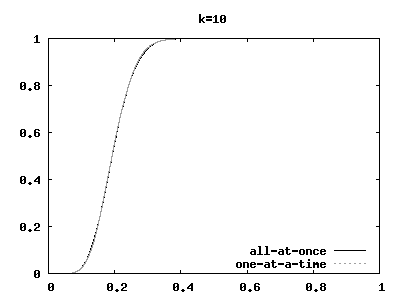
\includegraphics[width=7.7cm]{compOneAll10}
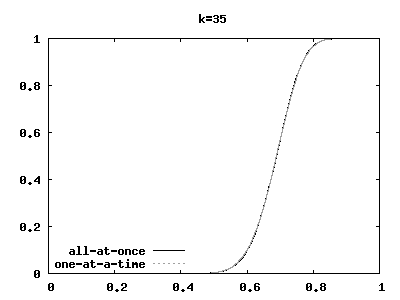
\includegraphics[width=7.7cm]{compOneAll35}
\vspace{-4mm}
\caption{Comparison of the distributions of arrival times generated using method 1 (all-at-once generation) and method 2 (once-at-a-time generation), for $k=10$ and $k=35$, $n=50$. }
\label{fig:compOneAll}
\vspace{-1mm}
\end{figure}
The match between the distributions contributes to the confirmation
that the two methods provide arrival times with similar distributions.
%
%
\subsubsection{Comparison of the One-at-a-Time Generated Samples and the Theoretical Distribution of Order Statistics}
The purpose of this section is to provide a comparison between the
empirical distribution of the $x_{(k)}$'s generated by the method
described in section~\ref{sec:methodtwo} (one-at-a-time generation)
and the theoretical distribution of the $k$-th order
statistics. Section~\ref{sec:proof} proves that these two
distributions match, so this numerical comparison only comes as an
empirical confirmation.\par
The (theoretical) distribution $F_{X_{(k)}}$ of the $k$-th order
statistic can be determined, using
equation~(\ref{eq:densityOrder}). An integration by part provides the
following recursion formula for the probability distribution of the
order statistics:
\begin{equation}
F_{X_{(k+1)}}(x) = -\frac{x}{k} f_{X_{(k)}}(x) + F_{X_{(k)}}(x)
\end{equation}
A closed form for each $F_{X_{(k)}}(x)$ can be determined from this recursion
formula:
\begin{equation}\label{eq:distributionOrder}
F_{X_{(k)}}(x) = 1 - \sum_{j=0}^{k-1} \frac{n!}{k!(n-k)!}x^j(1-x)^{n-j}
\end{equation}
Let us again consider a sample size $n=50$. The comparison is performed
as follows:
\begin{enumerate}
\item Generate a large number $N^\text{trials}$ of samples
  $(x^j_{(1)},\ldots,x^j_{(n)})$, where the index $j$ denotes the
  ``trial'' number, going from 1 to $N^\text{trials}$ (for each $j$,
  the one-at-a-time generation described in~\ref{sec:methodtwo} is
  performed).
\item For each $k$, determine the distribution of
  $\{x^1_{(k)},\ldots,x^{N^\text{trials}}_{(k)}\}$ (i.e., the $k$-th
  smallest value of each ``trial'').
\item For each $k$, plot the empirical distribution determined above,
  along with the theoretical distribution from
  equation~(\ref{eq:distributionOrder}).
\end{enumerate}
Figure~\ref{fig:compOneDistrib} shows a perfect match for these plots
for $k=10$ and $k=35$, with $N^\text{trials}=10,000$ trials.
\begin{figure}[ht]
\vspace{-3mm}
\centering
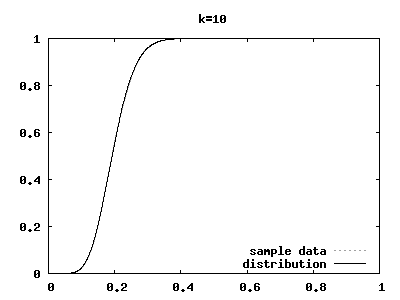
\includegraphics[width=7.7cm]{compOneDistrib10}
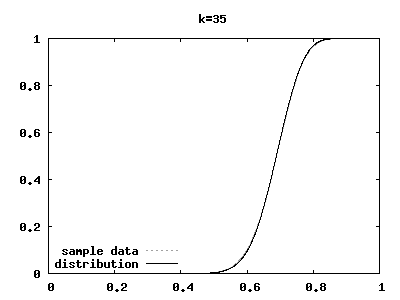
\includegraphics[width=7.7cm]{compOneDistrib35}
\vspace{-4mm}
\caption{Comparison of one-at-a-time generation and theoretical distribution of order statistics for $k=10$ (left) and $k=35$ (right), $n=50$.}
\label{fig:compOneDistrib}
\vspace{-4mm}
\end{figure}
%
%
%
\bibliographystyle{plainnat}
\bibliography{unif}
%
\begin{comment}
{\large One-at-a-Time Generation of Arrival Times in Increasing Order When the Number of Arrivals is Given and Arrivals Follow a Given Arrival Pattern}}
% Document Control
{\bfseries Document Control}\par\bigskip
{\footnotesize
\begin{tabular}{|p{2cm}|p{2cm}|p{3cm}|p{3cm}|p{3.5cm}|}
\hline
{\bfseries Security level} & \multicolumn{4}{l|}{%
% Security Level
}
\\\hline
{\bfseries Company} & \multicolumn{4}{l|}{%
% Company
Amadeus SAS}
\\\hline
{\bfseries Department} & \multicolumn{4}{l|}{%
% Department
DEV-ORI-MSC}
\\\hline
{\bfseries Author} & \multicolumn{4}{l|}{%
% Author
Charles-Antoine Robelin}
\\\hline
{\bfseries Reviewed by} & \multicolumn{2}{l|}{%
% Reviewed by
%Fran\c{c}ois Laburthe
}
& {\bfseries Date} &
% Review Date
{}
\\\hline
{\bfseries Approved by} & \multicolumn{2}{l|}{%
% Approved by
%Fran\c{c}ois Laburthe
}
& {\bfseries Date} &
% Approval Date
{}
\\\hline
{\bfseries Version} & {\bfseries Date} & {\bfseries Change} & {\bfseries Comment} & {\bfseries By}
\\\hline
{0.1} % version
&
{31/05/2011} % date
&
{} % change
&
{} % comment
&
{Charles-Antoine Robelin } % by
\\\hline
{} % version
&
{} % date
&
{} % change
&
{} % comment
&
{} % by
\\\hline
\end{tabular}
}
\end{comment}
\end{document}
